%做功
\documentclass[11pt,tikz,border=3.14mm]{standalone}
\usepackage{pgfplots}
\pgfplotsset{compat=1.17}

\usepackage{xcolor}
\definecolor{r1}{HTML}{FF8674}
\definecolor{b1}{HTML}{17ABDD}
\definecolor{p1}{HTML}{D4B6D6}
\definecolor{g1}{HTML}{70E2CB}
\definecolor{o1}{HTML}{DFA743}

\begin{document}
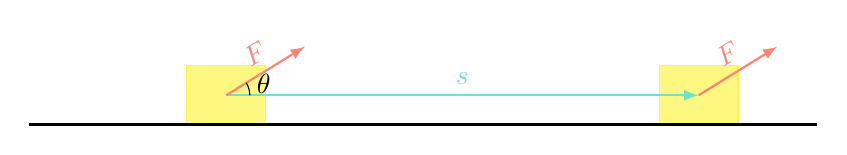
\begin{tikzpicture}
	\draw [fill = yellow!50,draw = yellow!70] (-2,0) rectangle (-3,0.75);
	\draw [fill = yellow!50,draw = yellow!70] (3,0) rectangle (4,0.75);
	\draw [very thick] (-5,0)--(5,0);
	\draw [-latex,thick,g1] (-2.5,0.375) -- (3.5,0.375) node[midway,above]{$s$};
	\draw [-latex,thick,r1] (-2.5,0.375) -- (-1.5,0.993) node[midway, sloped, above]{$F$};
	\draw [-latex,thick,r1] (3.5,0.375) -- (4.5,0.993) node[midway, sloped, above]{$F$};
	\draw (-2.2,0.375) arc (0:31.71:0.3) node[very near end, right ]{$\theta$};
\end{tikzpicture}


\end{document}